\documentclass{article}

% if you need to pass options to natbib, use, e.g.:
% \PassOptionsToPackage{numbers, compress}{natbib}
% before loading nips_2017
%
% to avoid loading the natbib package, add option nonatbib:
% \usepackage[nonatbib]{nips_2017}


% to compile a camera-ready version, add the [final] option, e.g.:
% \usepackage[final]{nips_2017}

\usepackage[final]{nips_2018}

\usepackage{placeins}
\usepackage[utf8]{inputenc} % allow utf-8 input
\usepackage[T1]{fontenc}    % use 8-bit T1 fonts
\usepackage{hyperref}       % hyperlinks
\usepackage{url}            % simple URL typesetting
\usepackage{booktabs}       % professional-quality tables
\usepackage{amsfonts}       % blackboard math symbols
\usepackage{nicefrac}       % compact symbols for 1/2, etc.
\usepackage{microtype}      % microtypography
\usepackage{graphicx}

\title{COMP 4211 - Machine Learning Programming Assignment 2 Report}

\author{%
	Cheng Chi Fung \\
	\texttt{cfchengac@connect.ust.hk} \\
}

\begin{document}

\maketitle

\section{CNN Classifier}

\subsection{Screen Shots of the CNN Classifier}
The following are the screen shot of the CNN Network and loading the pretrained encoder.

\begin{figure}[h]
  \centering
  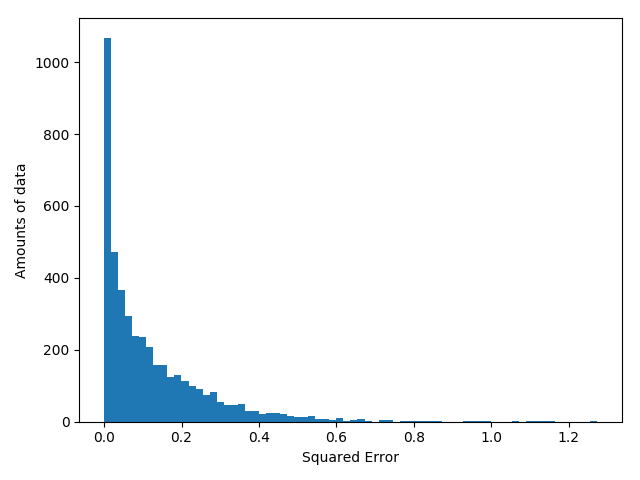
\includegraphics[scale=0.3]{fifa_lg.png}
  \caption{Screen shot of the CNN Network}
\end{figure}

\begin{figure}[h]
  \centering
  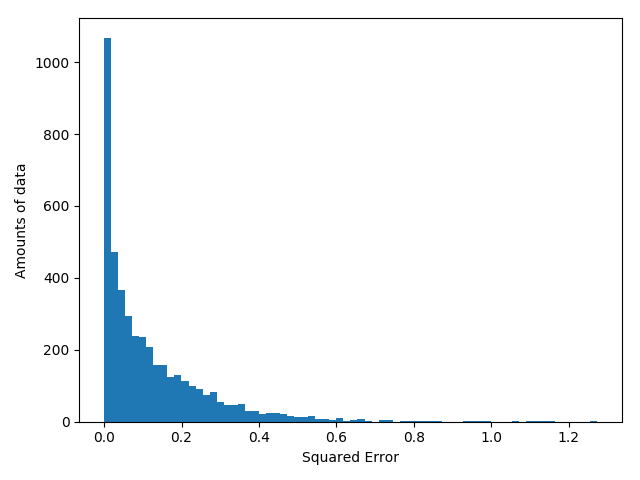
\includegraphics[scale=0.3]{fifa_lg.png}
  \caption{Screen Loading the Pretrained Encoder}
\end{figure}
\subsection{Hold out validation result of CNN classifier from scratch}

The following are the hold out validation results of CNN classifier from scratch. The network archiecture of using in the hold out validation was the same as the snapshot above. In the validation, we partitioned the training set into the training and validation sets with ratio 4:1. For each candidate set of hyperparameters, we trained the network for $20$ epochs batch size $32$ and validate it against the validation set. The cross entropy loss shown in the results table was the optimal one .

\pagebreak

\begin{table}[htb]
\caption{Hold out Validation Results of scratch CNN classifer}
	\label{sample-table}
	\centering
\begin{tabular}{lllll}
\toprule
		\cmidrule{1-5}
		Parameters set& Optimizer & Learning Rate & Num of Hidden & Cross Entropy Loss 		\\
		\midrule
 			1 & Adam & 0.001 & 32 & awd \\
 			2 & SGD & 0.1 & 32 &  wd\\
 			3 & SGD & 0.01 & 32 & wd \\
			4 & Adam & 0.001 & 64 & wd \\
 			5 & SGD & 0.1 & 64 &  wd\\
 			6 & SGD & 0.01 & 64 & dw \\
\bottomrule
\end{tabular}
\end{table}

The cross entropy loss of parameters set x had the lowest optimal cross entropy loss after conducting the hold out validation, so we would choose the parameters set [Adam, 0.001, 32] as the hyperparameters for the training in the testing phase.


\subsection{Hold out validation result of the CNN classifier with Pretrained Encoder Weights}

The following are the hold out validation results of the CNN classifier with pretrained encoder weights. The network archiecture of using in the hold out validation was the same as the snapshot above. In the validation, we partitioned the training set into the training and validation sets with ratio 4:1. For each candidate set of hyperparameters, we trained the network for $20$ epochs batch size $32$ and validate it against the validation set. The cross entropy loss shown in the results table was the optimal one .


\begin{table}[htb]
\caption{Hold out Validation Results of scratch CNN classifer}
	\label{sample-table}
	\centering
\begin{tabular}{lllll}
\toprule
		\cmidrule{1-5}
		Parameters set& Optimizer & Learning Rate & Num of Hidden & Cross Entropy Loss 		\\
		\midrule
 			1 & Adam & 0.001 & 32 & awd \\
 			2 & SGD & 0.1 & 32 &  wd\\
 			3 & SGD & 0.01 & 32 & wd \\
			4 & Adam & 0.001 & 64 & wd \\
 			5 & SGD & 0.1 & 64 &  wd\\
 			6 & SGD & 0.01 & 64 & dw \\
\bottomrule
\end{tabular}
\end{table}

The cross entropy loss of parameters set x had the lowest optimal cross entropy loss after conducting the hold out validation, so we would choose the parameters set [Adam, 0.001, 32] as the hyperparameters for the training in the testing phase.


\subsection{Testing Results of CNN Classifier}

In the testing phase, for both CNN classifier from scratch and with Pretrained Encoder Weights, we trained using the entire training set with the best set of hyperparameters obtained from the hold out validation and the same network architecture as the hold out validation, and tested with the testing test. We used $32$ as our batch size and trained with $20$ epoch. The following was the results obtained from the testing phase.

\begin{table}[htb]
\caption{Testing Result Metric of CNN classifier from scratch}
	\label{sample-table}
	\centering
\begin{tabular}{llll}
\toprule
		\cmidrule{1-4}
		& Cross Entropy Loss & Top-1 Accuracy & Top-3 Accuracy 		\\
	\midrule
 	Mean & SGD & 0.1 & 32 \\
 	Std & SGD & 0.1 & 32\\
\bottomrule
\end{tabular}
\end{table}

\begin{table}[htb]
\caption{Testing Result Metric of CNN classifier with Pretrained Encoder Weights}
	\label{sample-table}
	\centering
\begin{tabular}{llll}
\toprule
		\cmidrule{1-4}
		& Cross Entropy Loss & Top-1 Accuracy & Top-3 Accuracy 		\\
	\midrule
 	Mean & SGD & 0.1 & 32  \\
 	Std & SGD & 0.1 & 32 \\
\bottomrule
\end{tabular}
\end{table}

\pagebreak

\begin{figure}[h]
  \centering
  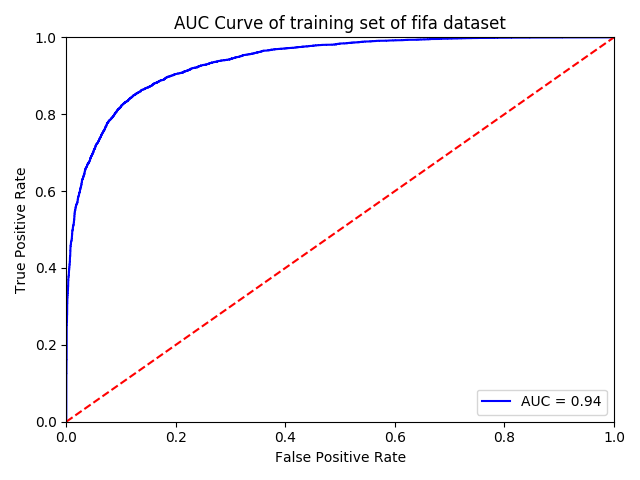
\includegraphics[scale=0.3]{fifa_auc_train.png}
  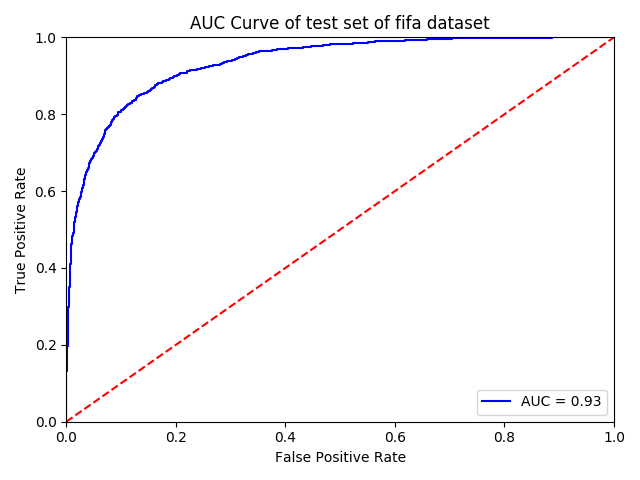
\includegraphics[scale=0.3]{fifa_auc_test.png}
  \caption{Learning Curve of Cross Entropy Loss}
\end{figure}

\FloatBarrier


\begin{figure}[h]
  \centering
  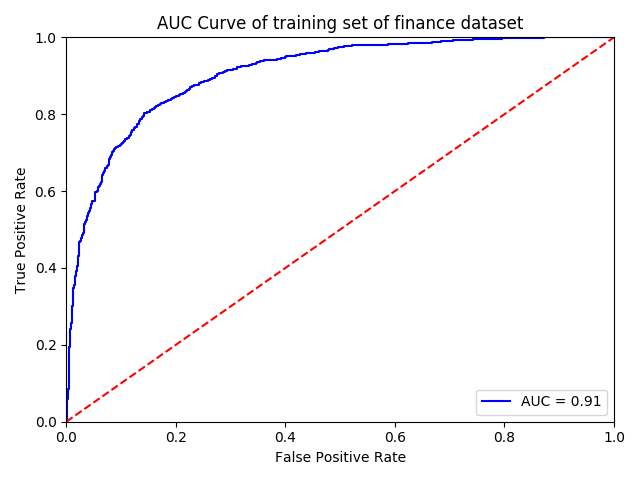
\includegraphics[scale=0.3]{finance_auc_train.png}
  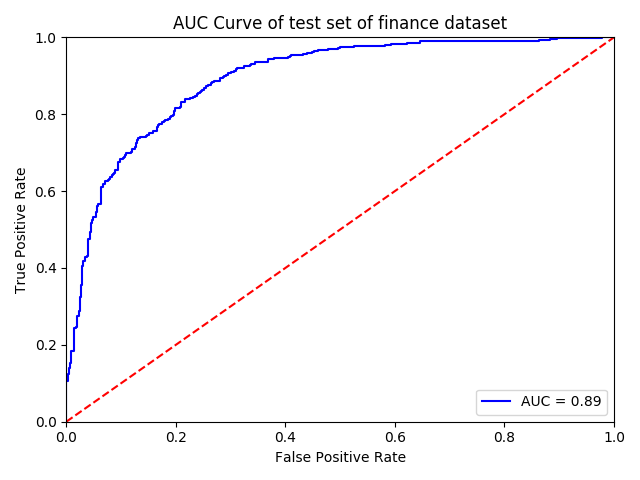
\includegraphics[scale=0.3]{finance_auc_test.png}
  \caption{Learning Curve of Top-1 Accuracy}
\end{figure}

\pagebreak

\begin{figure}[h]
  \centering
  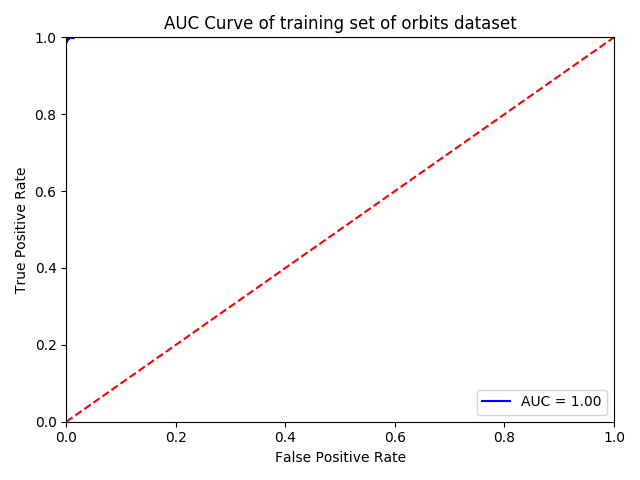
\includegraphics[scale=0.3]{orbits_auc_train.png}
  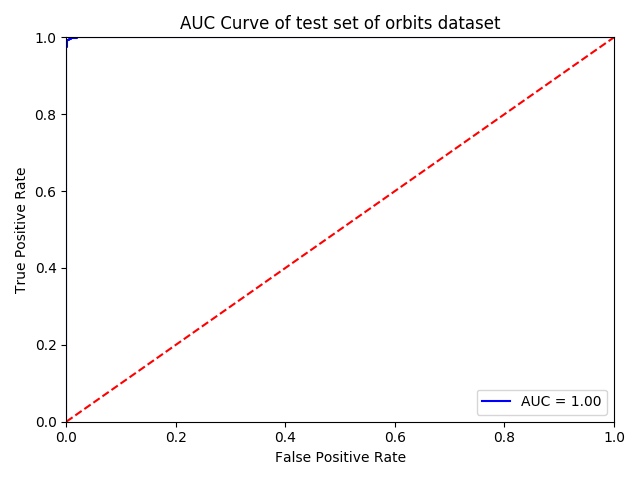
\includegraphics[scale=0.3]{orbits_auc_test.png}
  \caption{Learning Curve of Top-3 Accuracy}
\end{figure}

From the square loss histogram of test sets, we found out that the mean squared error of the most of the data points are around zero. It means that this model perform quite well for most of the data points. However, for the finance datasets, there are some data points that have the sqaured error far away from zero ($23.77581$) which means that there might be some \textbf{outliers} that far away from the curve.

\section{CAE with Pretrained Encoder}

\subsection{Screen Shots of the CAE with Pretrained Encoder}
The following are the screen shot of the Network of CAE Decoder and loading the pretrained encoder.

\begin{figure}[h]
  \centering
  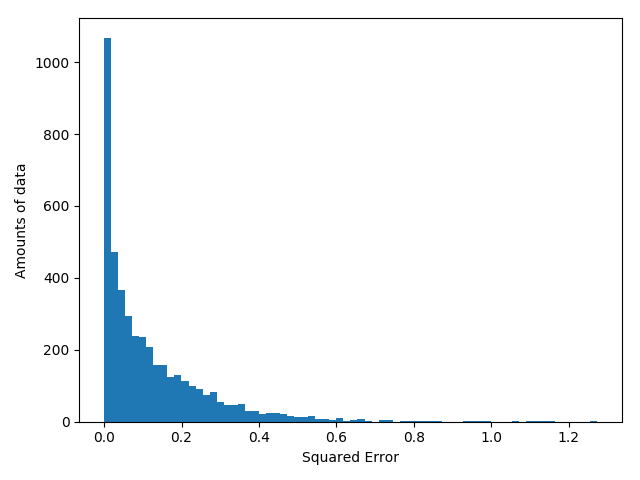
\includegraphics[scale=0.3]{fifa_lg.png}
  \caption{Screen shot of the Network of CAE Decoder}
\end{figure}

\begin{figure}[h]
  \centering
  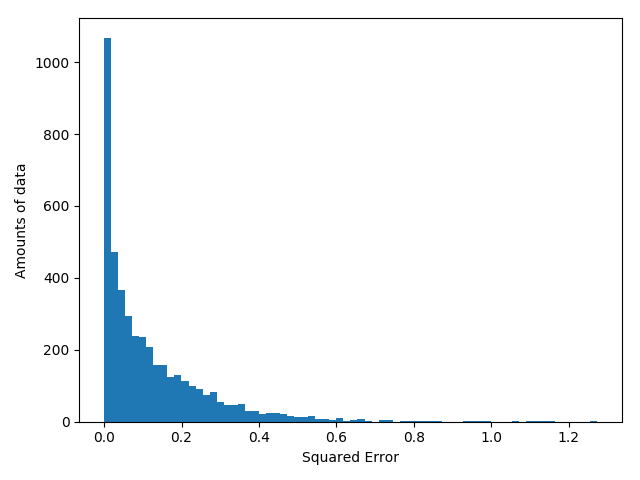
\includegraphics[scale=0.3]{fifa_lg.png}
  \caption{Screen Loading the Pretrained Encoder}
\end{figure}

\subsection{Hold out validation result of CAE with Pretrained Encoder}

The following are the hold out validation results of the CAE with Pretrained Encoder. The network archiecture of using in the hold out validation was the same as the snapshot above. In the validation, we partitioned the training set into the training and validation sets with ratio 4:1. For each candidate set of hyperparameters, we trained the network for $20$ epochs batch size $32$ and validate it against the validation set. The cross entropy loss shown in the results table was the optimal one .


\begin{table}[htb]
\caption{Hold out Validation Results of scratch CNN classifer}
	\label{sample-table}
	\centering
\begin{tabular}{lllll}
\toprule
		\cmidrule{1-5}
		Parameters set& Optimizer & Learning Rate & Num of Hidden & Cross Entropy Loss 		\\
		\midrule
 			1 & Adam & 0.001 & 32 & awd \\
 			2 & SGD & 0.1 & 32 &  wd\\
 			3 & SGD & 0.01 & 32 & wd \\
			4 & Adam & 0.001 & 64 & wd \\
 			5 & SGD & 0.1 & 64 &  wd\\
 			6 & SGD & 0.01 & 64 & dw \\
\bottomrule
\end{tabular}
\end{table}

\begin{figure}[h]
  \centering
  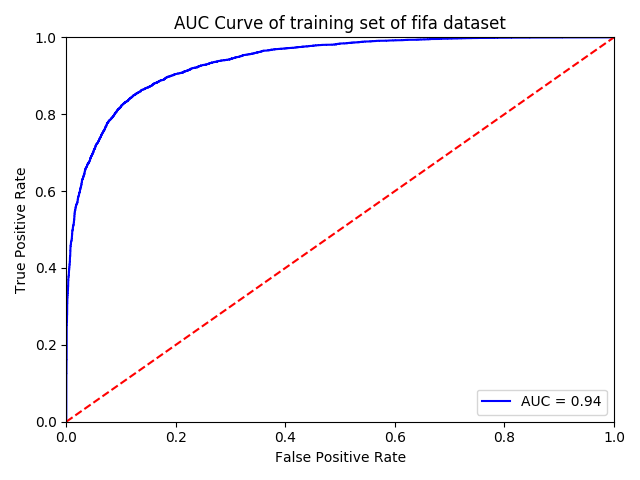
\includegraphics[scale=0.3]{fifa_auc_train.png}
  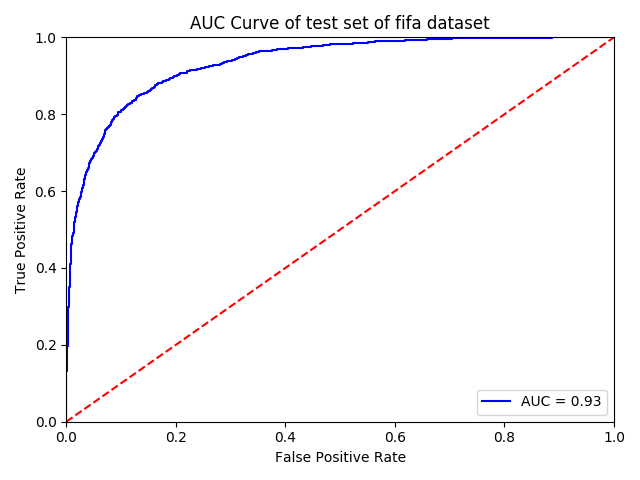
\includegraphics[scale=0.3]{fifa_auc_test.png}
  \caption{Learning Curve of Cross Entropy Loss}
\end{figure}

\FloatBarrier


\begin{figure}[h]
  \centering
  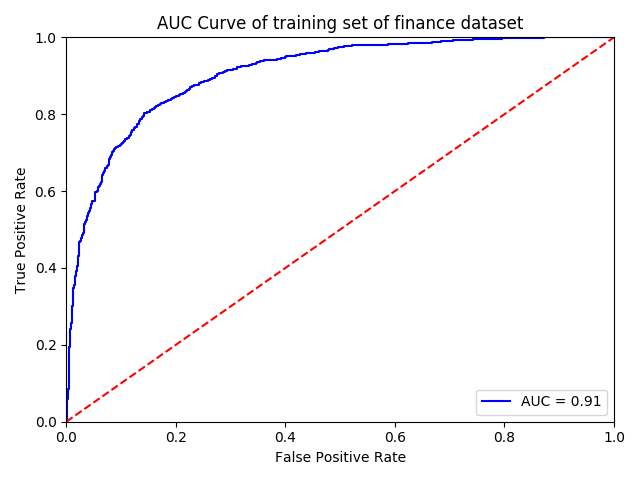
\includegraphics[scale=0.3]{finance_auc_train.png}
  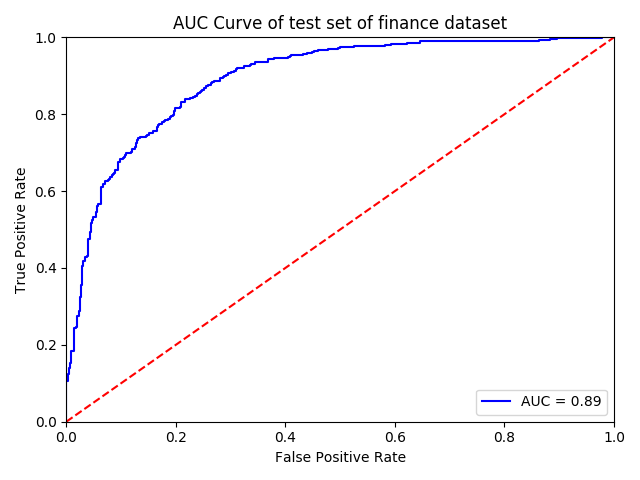
\includegraphics[scale=0.3]{finance_auc_test.png}
  \caption{Learning Curve of Top-1 Accuracy}
\end{figure}

\pagebreak

\begin{figure}[h]
  \centering
  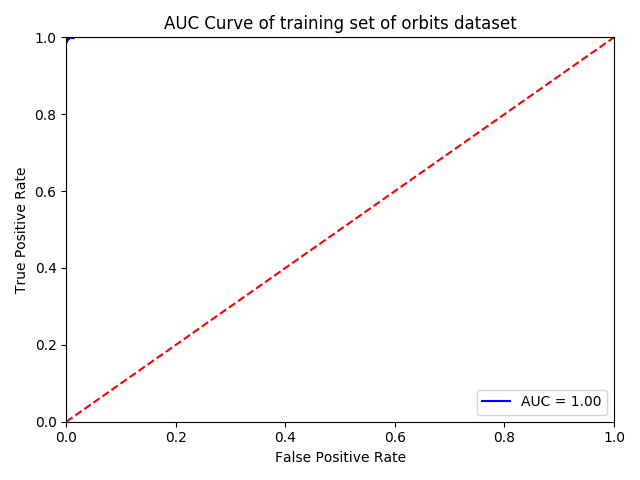
\includegraphics[scale=0.3]{orbits_auc_train.png}
  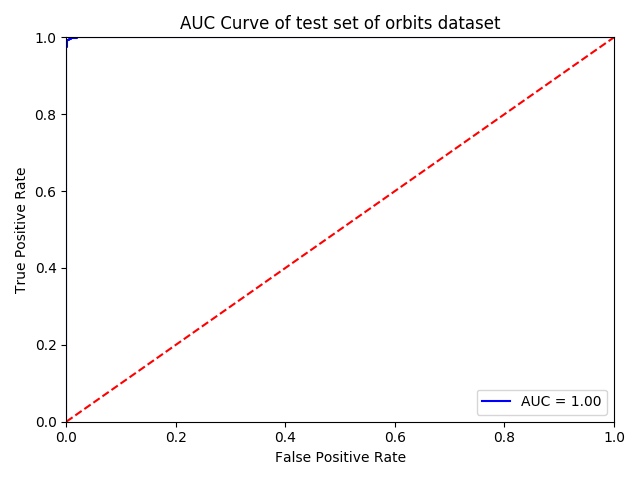
\includegraphics[scale=0.3]{orbits_auc_test.png}
  \caption{Learning Curve of Top-3 Accuracy}
\end{figure}

The cross entropy loss of parameters set x had the lowest optimal cross entropy loss after conducting the hold out validation, so we would choose the parameters set [Adam, 0.001, 32] as the hyperparameters for the training in the testing phase.

\subsection{Testing Results of CAE with Pretrained Encoder}

In the testing phase, for both CNN classifier from scratch and with Pretrained Encoder Weights, we trained using the entire training set with the best set of hyperparameters obtained from the hold out validation and the same network architecture as the hold out validation, and tested with the testing test. We used $32$ as our batch size and trained with $20$ epoch. The following was the results obtained from the testing phase.

\begin{table}[htb]
\caption{Testing Result Metric of CNN classifier from scratch}
	\label{sample-table}
	\centering
\begin{tabular}{llll}
\toprule
		\cmidrule{1-4}
		& Cross Entropy Loss & Top-1 Accuracy & Top-3 Accuracy 		\\
	\midrule
 	Mean & SGD & 0.1 & 32 \\
 	Std & SGD & 0.1 & 32\\
\bottomrule
\end{tabular}
\end{table}


\pagebreak

\begin{figure}[h]
  \centering
  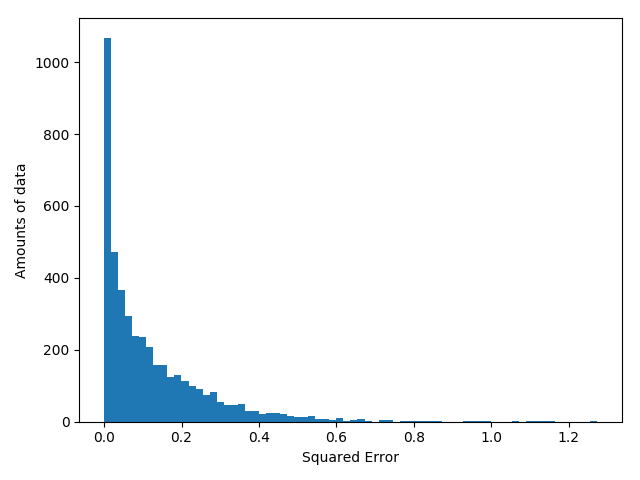
\includegraphics[scale=0.3]{fifa_lg.png}
  \caption{Screen shot of the CNN Network}
\end{figure}

\begin{figure}[h]
  \centering
  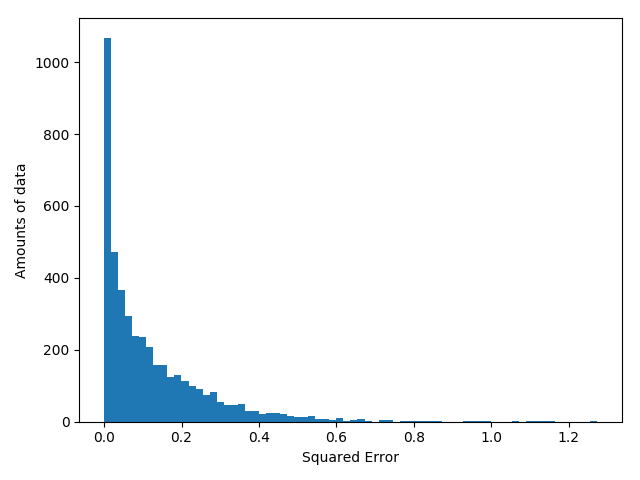
\includegraphics[scale=0.3]{fifa_lg.png}
  \caption{Screen shot of the CNN Network}
\end{figure}


From the square loss histogram of test sets, we found out that the mean squared error of the most of the data points are around zero. It means that this model perform quite well for most of the data points. However, for the finance datasets, there are some data points that have the sqaured error far away from zero ($23.77581$) which means that there might be some \textbf{outliers} that far away from the curve.

\end{document}

